\documentclass{beamer}

\mode<presentation>
{
  \usetheme{default}
  \setbeamertemplate{navigation symbols}{}
  \setbeamertemplate{footline}[frame number]
  \setbeamertemplate{items}[circle]
  \usecolortheme{seahorse}
}

\usepackage[english]{babel}
\usepackage[utf8]{inputenc}
\usepackage{times}
\usepackage[T1]{fontenc}

\title[Lost!] % (optional, only for long titles)
{Lost in Space}
\subtitle{Binary search trees beyond dimension one}

\author[Abrahamson]
{Jeff Abrahamson}
\institute[Google]{Google, Inc.}

\date[Big-O Meetup]
{London Big-O Meetup, 21 May 2014}

\subject{kd-trees, range trees, and other generalizations of BST's}
% This is only inserted into the PDF information catalog. Can be left
% out.

% Delete this, if you do not want the table of contents to pop up at
% the beginning of each subsection:
\AtBeginSubsection[]
{
  \begin{frame}<beamer>{Outline}
    \tableofcontents[currentsection,currentsubsection]
  \end{frame}
}

% If you wish to uncover everything in a step-wise fashion, uncomment
% the following command: 
%\beamerdefaultoverlayspecification{<+->}

\begin{document}

% \frame{\titlepage}

\begin{frame}
  \titlepage
\end{frame}

\begin{frame}
  \frametitle{Outline}
  \tableofcontents[pausesections]
\end{frame}

\section{$\mathbb{R}^1$}
\subsection{BST}

\begin{frame}
  \frametitle{Binary Search Trees}
  \begin{itemize}
  \item Is $p\in S$?
  \item Given $x$, what is closest point $p\in S$?
  \item Find $\{x\,|\,x \textrm{ is in the interval between } p_1 \textrm{ and } p_2\}$.
  \item Given $\delta$, find $\{x\,|\,\mathrm{d}(x,p) < \delta\}$.
  \end{itemize}
  \pause
  \bigskip
  \textcolor{blue}{This is easy in $\mathbb{R}^1$.  What about $\mathbb{R}^d$?}
\end{frame}
\note{Everyone knows about BST's?}
\note{How do we interpret these statements in $\mathbb{R}^d$?}

\section{$\mathbb{R}^d$}
\subsection{What could go wrong?}

\begin{frame}
  \frametitle{What could go wrong?}
  \textcolor{red}{The Curse of Dimensionality}\\
  \bigskip
  \pause
  Some things to think about:
  \begin{itemize}
  \item Volume of unit cube $\pm\epsilon$
  \item Distance from $(0,0,\ldots,0)$ to $(1,1,\ldots,1)$
  \end{itemize}
  \pause
  \bigskip
  \textcolor{blue}{It's easy to get lost.}
\end{frame}
\note{In Hilbert space, you can't even scream.}

\subsection{Quadtrees}

\begin{frame}
  \frametitle{Quadtrees in Words}
  Properties (let's start in $\mathbb{R}^2$)
  \begin{itemize}
  \item Rooted tree
  \item Internal nodes have four children
  \end{itemize}
\end{frame}

\begin{frame}
  \frametitle{Quadtrees in Pictures}
  % Rather than xfig, probably I should use TikZ and PGF.
  % Cf. http://www.texample.net/tikz/examples/
  \includegraphics<1->[width=.45\textwidth]{quad-tree-squares.pdf}\hfill
  \includegraphics<2>[width=.45\textwidth]{quad-tree-tree.pdf}
\end{frame}

\begin{frame}
  \frametitle{Quadtrees in Mathematics}
  \begin{itemize}
  \item Find a bounding box: $O(n)$
  \item Then,
    \begin{itemize}
    \item Divide in four quadrants: $O(1)$
    \item Partition the points: $O(n)$
    \item Recursively build a quad tree: ??
    \end{itemize}
  \end{itemize}
\end{frame}

\begin{frame}
  \frametitle{Quadtrees in Equations}
  
  \begin{itemize}
  \item Depth is at most $\delta = \left\lceil
      \log\left(\frac{s}{c}\right) +
      \frac{3}{2}\right\rceil$\textcolor{gray}{, where $c$ is the
      smallest inter-point distance and $s$ is the side length of the
      initial square.} \\[2mm]
    
  \item \textcolor{gray}{A quadtree of depth $\delta$ storing $n$ points has}
    $O((\delta+1)n)$ nodes and requires $O((\delta+1)n)$ time to
    construct. \\[2mm]
    
  \item Finding neighbors \textcolor{gray}{in a given direction takes}
    time $O(\delta+1)$ \\[2mm]

  \item Balancing \textcolor{gray}{a quadtree takes} time
    $O((\delta+1)m)$\textcolor{gray}{, where $m$ is the number of
      interior nodes.}

  \end{itemize}
\end{frame}
\note{But depth is kinda sorta $\log(n)$, so we're in $n\log(n)$ land.}

\begin{frame}
  \frametitle{Quadtrees in Popular Culture}

  \begin{itemize}
  \item One of the first DS's for higher-dimensional data
  \item Finkel and Bentley, 1974
    \textcolor{gray}{\small\it(R.~A.~Finkel and J.~L.~Bentley, Quad
      trees: a data structure for retrieval on composite keys. Acta
      Inform, 4:1--9, 1974)}
  \item Still perform relatively well
  \item Easy to generalize to higher dimensions---called octrees
  \end{itemize}

  \bigskip \textcolor{gray}{M. de Berg et al., \textit{Computational
      Geometry: Algorithms and Applications}, second edition, chapter
    14.  Cf. also chapter end notes.}
\end{frame}

\subsection{kd-trees}

\begin{frame}
  \frametitle{Kd-Trees in Words}
  \begin{itemize}
  \item Range queries
    \pause
  \item Data bases!  Records are points in space.
  \end{itemize}
\end{frame}

\begin{frame}
  \frametitle{Kd-Trees in SQL}

  Find employees who are past their trial period but in their first
  year and who are close to hitting the \pounds 100K tax rule start.

  \bigskip

  \texttt{SELECT salary, hire$\_$date\\
  FROM EMPLOYEES\\
  WHERE 80000 < salary AND salary < 100000\\
  AND 3m < hire$\_$date AND hire$\_$date < 12m}
\end{frame}

\begin{frame}
  \frametitle{Kd-Trees in Pictures}

  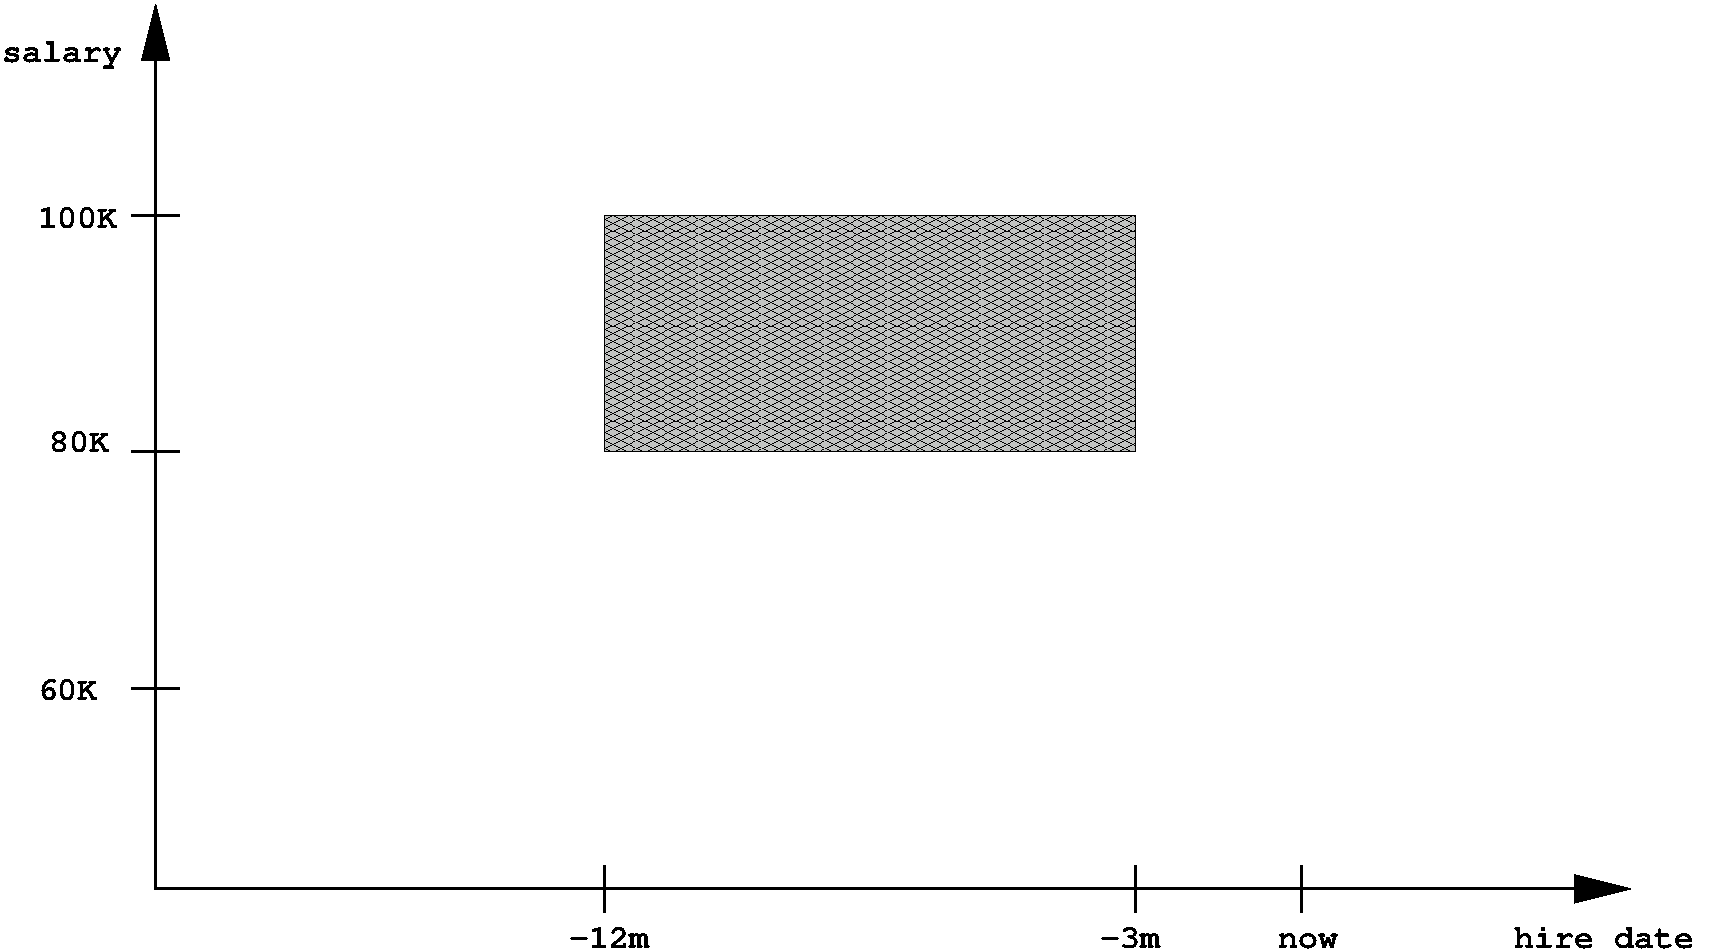
\includegraphics[width=\textwidth]{kd-SQL.pdf}
\end{frame}

\begin{frame}
  \frametitle{Kd-Trees in $\mathbb{R}^1$}
  
  \begin{itemize}
  \item Binary search tree
  \item Find beginning of range
  \item Tree walk to end of range
  \end{itemize}
\end{frame}

\begin{frame}
  \frametitle{Kd-Trees in $\mathbb{R}^2$}
  \begin{itemize}
  \item At root, start with all points.
  \item Partition on $x$ value to make level 1 nodes
  \item Partition those sets on $y$ value to make level 2 nodes
  \item Repeat until done
  \end{itemize}
\end{frame}

\begin{frame}
  \frametitle{Kd-Trees in Pictures}

  \includegraphics<1>[width=.45\textwidth]{kd-tree-0.pdf} 
  \includegraphics<1>[width=.45\textwidth]{kd-tree-graph-0.pdf}
%
  \includegraphics<2>[width=.45\textwidth]{kd-tree-1.pdf}
  \includegraphics<2>[width=.45\textwidth]{kd-tree-graph-1.pdf}
%
  \includegraphics<3>[width=.45\textwidth]{kd-tree-2.pdf}
  \includegraphics<3>[width=.45\textwidth]{kd-tree-graph-2.pdf}
%
  \includegraphics<4>[width=.45\textwidth]{kd-tree-3.pdf}
  \includegraphics<4>[width=.45\textwidth]{kd-tree-graph-3.pdf}
%
  \includegraphics<5>[width=.45\textwidth]{kd-tree-4.pdf}
  \includegraphics<5>[width=.45\textwidth]{kd-tree-graph-4.pdf}
%
  \includegraphics<6>[width=.45\textwidth]{kd-tree-full.pdf}
  \includegraphics<6>[width=.45\textwidth]{kd-tree-graph-5.pdf}
  
\end{frame}

\begin{frame}
  \frametitle{Kd-Trees}
  \begin{itemize}
  \item 
  \end{itemize}
\end{frame}

\begin{frame}
  \frametitle{Kd-Trees}
  \begin{itemize}
  \item 
  \end{itemize}
\end{frame}

\begin{frame}
  \frametitle{Kd-Trees}
  \begin{itemize}
  \item 
  \end{itemize}
\end{frame}

\subsection{Range trees}

\begin{frame}
  \frametitle{Range trees}
  \dots
\end{frame}

\subsection{More}

\begin{frame}
  \frametitle{More\dots}
  \begin{itemize}
  \item Voronoi diagrams
  \item database range searches
  \item Trees in the forest
  \item Other applications
  \item What if we want to insert or delete points?
  \end{itemize}
\end{frame}

\section*{Summary}

\begin{frame}
  \frametitle{Summary}  
  \dots
\end{frame}

\begin{frame}
  \frametitle{Questions}  
\end{frame}

\end{document}
